\documentclass{article}

\usepackage{amsmath}
\usepackage{palatino}
\usepackage{tikz}

\begin{document}
\begin{enumerate}
\item[1.3.1]
  To show that the epimorphisms in \textbf{Set} are the surjective functions, let $f : A \rightarrow B$ be a surjective function and let $g : B \rightarrow C$ and $h : B \rightarrow C$ be other arrows in \textbf{Set}.
  First, assume both that $g$ and $h$ are equal and that $g \circ f \ne h \circ f$ to derive a contradiction.
  Let $x$ be an element of $A$ such that $g(f(x)) \ne h(f(x))$.
  If $f(x) = y$ we have that $g(y) \ne h(y)$, but this contradicts the assumption that $g$ and $h$ are equal.

  For the converse, assume that $g \circ f = h \circ f$ but that $g \ne h$.
  The first equality states that $\forall x\in A~.~g(f(x)) = h(f(x)) \rightarrow g(y) = h(y)$ if $y = f(x)$.
  Because $f$ is surjective, this derivation shows that $g$ and $h$ agree on all elements of their common domain, thus contradicting the assumption that $g \ne h$.

\item [1.3.2]
  To show that the composition of two monic arrows is monic, let $f : B \rightarrow C$ and $g : C \rightarrow D$ be monic arrows.
  First, let $a : A \rightarrow B$ and $b : A \rightarrow B$ be two equal arrows.
  We derive $(g \circ f) \circ a = (g \circ f) \circ b$ by assuming there is some element $x \in A$ for which the equality does not hold.

  By the equality of $a$ and $b$, we know that $(g\circ f)(a(x)) \ne (g\circ f)(b(x)) \Rightarrow (g\circ f)(y) \ne (g\circ f)(y)$ for a $y = a(x) = b(x)$.
  This implies $g(f(y)) \ne g(f(y))$, a contradiction.

  Next, assume that $(g\circ f) \circ a = (g\circ f) \circ b$ but that $a \ne b$.
  Then we have some element $x \in A$ such that $a(x) = y_1 \ne y_2 = b(x)$.
  This implies that $g(f(y_1)) = g(f(y_2))$.
  However, $g$ is a monomorphism and $f$ is equal to itself, so we arrive at a contradiction.

  For the second part, let $f : B \rightarrow C$ and $g : C \rightarrow D$ be functions such that $(g \circ f) : B \rightarrow D$ is monic.
  Then for functions $a,b : A \rightarrow B$, $(g \circ f) \circ a = (g \circ f) \circ b$ implies $a = b$.
  We see that $f$ must be monic because the domain of $f$ is equal to the domain of $(g \circ f)$ and the codomains of $a$ and $b$.
  If $f$ were not monic then our assumption could not hold.

\item[]
\item[1.3.3]
  Let $f$ and $g$ be epic functions.
  We see that their composition $g \circ f$ must also be epic by associativity of $\circ$.
  The equality $a \circ (g \circ f) = b \circ (g \circ f)$ may be parenthesized as $(a \circ g) \circ f = (b \circ g) \circ f$.
  Because $f$ is epic, equality proves that $a \circ g = b \circ g$.
  Because $g$ is epic, equality here proves that $a = b$.
  Thus we have that $a \circ (g \circ f) = b \circ (g \circ f)$ implies $a = b$.

  Proving that if $(g \circ f)$ is epic then $g$ is epic follows a similar argument as used in the second part of 1.3.2.
  Namely, the codomain of $g$ is the same as the codomain of $(g \circ f)$.
  This observation leads to a similar contradiction as before; if $g$ were not epic then the statement $a \circ (g \circ f) = b \circ (g \circ f)$ implies $a = b$ would be false.

\item[]
\item[1.3.4]
  To show that the inverse $f^{-1} : B \rightarrow A$ of an isomorphism $f : A\rightarrow B$ is unique, assume the existence of a function $f^{-1}_2 : B \rightarrow A$ such that $f^{-1} \circ f = id_A = f^{-1}_2 \circ f$ and $f^{-1} \ne f^{-1}_2$.
  Let $y$ be an element of $B$ such that $f^{-1}(b) \ne f^{-1}_2(b)$, and let $x$ be the preimage of $b$ in $f$.
  Then we have $f^{-1}(f(x)) \ne f^{-1}_2(f(x)) \Rightarrow f^{-1}(y) \ne f^{-1}_2(y) \rightarrow x_1 \ne x_2$ for unequal elements $x_1,x_2 \in A$.
  However, if $x_1 \ne x_2$ then either (or both) of $x_1$ and $x_2$ cannot equal $x$.
  If $x_i = x$ does not hold, then the ``inverse'' function was incorrect; an isomorphism preserves identity.

\item[]
\item[1.3.5]
  We show that if $f : A \rightarrow B$ and $g : B \rightarrow C$ are isomorphisms then $g \circ f$ is an isomorphism with $f^{-1} \circ g^{-1}$ as its inverse.

  First, define objects $A$, $B$, and $C$.
  \begin{center}
    \begin{tikzpicture}
      \node (1) {$A$};
      \node[right of=1,xshift=1cm] (2) {$B$};
      \node[right of=2,xshift=1cm] (3) {$C$};
    \end{tikzpicture}
  \end{center}

  By definition, we have arrows $f : A \rightarrow B$ and $f^{-1} : B \rightarrow A$ such that $f^{-1} \circ f = id_A$.
  \begin{center}
    \begin{tikzpicture}
      \node (1) {$A$};
      \node[right of=1,xshift=1cm] (2) {$B$};
      \node[right of=2,xshift=1cm] (3) {$C$};

      \draw[->] (1) edge[bend left] node[above] {$f$} (2);
      \draw[->] (2) edge[bend left] node[below] {$f^{-1}$} (1);
    \end{tikzpicture}
  \end{center}

  Likewise, we have $g : B \rightarrow C$ and $g^{-1} : C \rightarrow B$ such that $g^{-1} \circ g = id_B$.
  \begin{center}
    \begin{tikzpicture}
      \node (1) {$A$};
      \node[right of=1,xshift=1cm] (2) {$B$};
      \node[right of=2,xshift=1cm] (3) {$C$};

      \draw[->] (2) edge[bend left] node[above] {$g$} (3);
      \draw[->] (3) edge[bend left] node[below] {$g^{-1}$} (2);
    \end{tikzpicture}
  \end{center}

  Together, these arrows yield the diagram:
  \begin{center}
    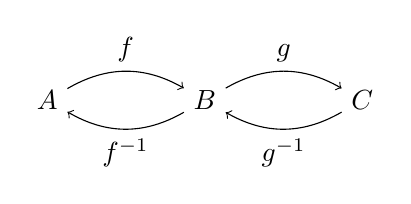
\begin{tikzpicture}
      \node (1) {$A$};
      \node[right of=1,xshift=1cm] (2) {$B$};
      \node[right of=2,xshift=1cm] (3) {$C$};

      \draw[->] (1) edge[bend left] node[above] {$f$} (2);
      \draw[->] (2) edge[bend left] node[below] {$f^{-1}$} (1);
      \draw[->] (2) edge[bend left] node[above] {$g$} (3);
      \draw[->] (3) edge[bend left] node[below] {$g^{-1}$} (2);
    \end{tikzpicture}
  \end{center}

  From which it is clear that $(f^{-1} \circ g^{-1}) \circ (g \circ f) = id_A$.

\item[]
\item[1.3.6] The category $\textbf{2}$ has an arrow, $f$, that is both a monomorphism and an epimorphism but not an isomorphism. 
  \begin{center}
  \begin{tikzpicture}[node distance=2cm, auto]
  \node (A) {$A$};
  \node (B) [right of=A] {$B$};
  \draw[->] (A) to node {$f$} (B);
  \end{tikzpicture}
  \end{center}
  This holds because of the limited number of compositions we can make. 
  Ignoring composition of identities, there are only two possibilities: $id_A;\ f$ and $f;\ id_B$. 
  Yet there is no arrow $f^{-1}: B \rightarrow A$, so $f$ is not an isomorphism.
\end{enumerate}
\end{document}
